Die in Abschnitt \ref{sub:problem} vorgestellte formale Definition des Problems versetzt uns in die Lage, vergleichsweise einfach ein Integer Linear Program anzugeben, das die gegebene Zielfunktion optimiert. Drei Variationen wollen wir im Folgenden vorstellen.

Allgemein haben wir uns entschieden, Kanten in diesen Modellen nicht zu berücksichtigen. Wir gehen davon aus, dass es möglich ist, bei ähnlichen Knotenpositionierungen auch ein ähnliches Kantenrouting zu finden. Dies wird vermutlich insbesondere dann einfacher, wenn die Kanten auch ursprünglich algorithmisch (und nicht manuell) geroutet worden sind. Für eine erste Idee, wie das Kantenrouting behandelt werden könnte, siehe Abschnitt \ref{sub:edgeroute}.

\subsection{Statische Reihenfolge}

Wir haben uns entschieden, neben der in \ref{eqn:opt:complete} formulierten Optimierungsfunktion noch etwas schärfere Maßstäbe anzulegen, und die horizontale und vertikale Reihenfolge der Knoten jedenfalls annähernd zu fixieren. Dies ergibt sich vor allem auch aus den in Abschnitt \ref{sub:tasks} gestellten Anforderungen. Als (horizontale oder vertikale) \textit{Reihenfolge} werden wir im Folgenden immer die Ordnung der Knoten entlang ihrer $x$- oder $y$-Koordinaten verstehen. Wir nennen zwei Knoten \textit{benachbart}, wenn sie in einer dieser Reihenfolgen aufeinander folgen.

Legt man sich fest, diese Reihenfolgen beim Finden eines neuen Layouts tatsächlich nicht zu verändern, und ist außerdem vorgegeben, an welcher Stelle der neue Knoten jeweils in die Reihenfolgen einzufügen ist, so lässt sich sogar ein Lineares Programm formulieren, das \ref{eqn:opt:complete} unter dieser Bedingung optimiert.\footnote{Andernfalls ist dies nicht möglich: Wenn es erlaubt ist, Knoten $A$ links oder rechts von $B$ zu platzieren, so ist die Bedingung zur Überlappungsfreiheit nicht ohne eine Integer-Variable zu formulieren.} Dieses LP hat nur eine Art von Nebenbedingungen, nämlich die, die für jedes Paar von (geometrisch) benachbarten Knoten die Überlappungsfreiheit sicherstellt. Dies ist eine starke Einschränkung: Prinzipiell ist es in einer gültigen Zeichnung erlaubt, dass zwei Knoten sich entweder horizontal oder vertikal überlappen, nicht jedoch beides. Im Linearen Programm muss nun festgelegt werden, in welcher Dimension zwei (benachbarte) Knoten sich nicht überlappen dürfen. Eine Formulierung "`Entweder horizontal oder vertikal"' ist ohne Integer-Variablen nicht möglich. Ansonsten können die Terme aus \ref{eqn:opt:complete} direkt als Optimierungsfunktion übernommen werden.

Eine interessante Beobachtung ist an dieser Stelle, dass wir zwei vollständige Ordnungen auf den Knoten definieren und erzwingen (eine horizontale und eine vertikale), während eventuell zwei Halbordnungen ausreichend wären: Für Knoten, die weit voneinander entfernt, und somit visuell nicht in einem Zusammenhang stehen, muss vermutlich nicht zwangsläufig festgelegt sein, in welcher Reihenfolge diese stehen. Genause verhält es sich mit Knoten, die einander horizontal oder vertikal überlappen: Aktuell legen wir hier willkürlich durch Wahl der linken oberen Ecke beziehungsweise durch ein Tie Breaking eine Reihenfolge fest, die vermutlich nicht zwangsläufig hilfreich ist. Um die Überlappungsfreiheit in einem LP gewährleisten zu können, ist dies allerdings notwendig.

\subsection{Begrenzte Vertauschungen}
\label{sub:ilp:2}

Im nächsten Schritt wollen wir nun einige Vertauschungen in der Reihenfolge der Knoten zulassen, allerdings nur Vertauschungen von jeweils 2 in der Reihenfolge unmittelbar benachbarten Knoten. Außerdem werden wir die Einschränkung aufheben, dass im Voraus festgelegt sein muss, ob zwei Knoten horizontal oder vertikal überlappen dürfen. Hierzu führen wir zunächst boolesche Indikatorvariablen $I^{v}_{i,j}$ und $I^{h}_{i,j}$ ein, die angeben, ob die Knoten $i$ und $j$ jeweils in der horizontalen bzw. vertikalen Ordnung vertauscht wurden. Diese Variablen existieren nur für den Fall, dass $i$ und $j$ in der entsprechenden Ordnung benachbart sind. Außerdem fügen wir pro Knotenpaar drei weitere Indikatorvariablen ein: Zunächst die Variable $D_{i,j}$, die die Richtung (horizontal oder vertikal) angibt, in der die beiden Knoten sich nicht überlappen dürfen. Außerdem fügen wir sowohl für die horizontale als auch die vertikale Überlappung die Variablen $O^{v}_{i,j}$ bzw. $O^{h}_{i,j}$ ein, die angibt, ob $i$ entlang der entsprechenden Achse vor oder hinter $j$ liegt. Seien $X_i$ und $Y_i$ die $X$- bzw. $Y$-Koordinate der linken oberen Ecke von $i$, und $w$ und $h$ die Höhe und Breite von $i$. Die Überlappungsfreiheit lässt sich nun formulieren als:

\begin{align}
	X_i + w_i &< X_j &&+ M \cdot D_{i,j} &+ M \cdot O^{h}_{i,j} \label{eqn:overlap:h1}\\
	X_i &> X_j + w_j &&- M \cdot D_{i,j} &- M + M \cdot O^{h}_{i,j} \label{eqn:overlap:h2}\\
	Y_i + h_i &< Y_j &&+ M - M \cdot D_{i,j} &+ M \cdot O^{v}_{i,j} \label{eqn:overlap:v1}\\
	Y_i &> Y_j + h_j &&- M + M \cdot D_{i,j} &- M + M \cdot O^{v}_{i,j} \label{eqn:overlap:v2}
\end{align}

Bei ausreichend groß gewähltem $M$ werden die Bedingungen \ref{eqn:overlap:h1} und \ref{eqn:overlap:h2} eingeschaltet, wenn eine horizontale Überlappung verboten werden soll, andernfalls sind  \ref{eqn:overlap:v1} und \ref{eqn:overlap:v2} aktiv. Innerhalb dieser Gruppen werden mittels $O^{h}_{i,j}$ bzw. $O^{v}_{i,j}$ je eine Bedingung ein- beziehungsweise ausgeschaltet.

Aufgrund dieser allgemeineren Bedingungen für die Überlappungsfreiheit müssen wir nun den Erhalt der Reihenfolge gesondert sicherstellen, falls zwei Knoten nicht vertauscht werden sollen. Für jedes Paar von benachbarten Knoten $i$ und $j$ fügen wir also eine Bedingung hinzu. Für ein horizontal benachbartes Paar, bei dem $i$ vor $j$ liegt beispielsweise:

\begin{align}
	X_i < X_j + M \cdot I^{h}_{i,j}
\end{align}

Welche Vertauschungen dies erlaubt, wird in Abbildung \ref{fig:neighbors} für die horizontale Reihenfolge deutlich: Die grünen, durchgezogenen Pfeile stellen hier erlaubte Vertauschungen dar, während die roten, gepunkteten Pfeile Beispiele für nicht erlaubte Vertauschungen darstellen. Wollte man beispielsweise Knoten $1$ und $3$ tauschen, so müsste Knoten $2$ in der horizontalen Reihenfolge "übersprungen" werden, was nicht erlaubt ist.

Auch wenn Vertauschungen hier in begrentztem Maß erlaubt sind, möchten wir die Anzahl der Vertauschungen nach wie vor minimieren, somit muss die Summe aller $I^{\{v,h\}}_{i,j}$ entsprechend gewichtet mit in die Optimierungsfunktion aufgenommen werden.

Dieser Ansatz erzeugt mit den Bedingungen zur Überlappungsfreiheit eine quadratische Anzahl von Nebenbedingungen und Integer-Variablen. In der Praxis (siehe Abschnitt \ref{sub:impl:opt}) können diese aber im Normalfall drastisch reduziert werden.

\subsection{Beliebige Vertauschungen}

Der naheliegende nächste Schritt ist es, beliebige Vertauschungen in der Reihenfolge zuzulassen. Nun werden also die Vertauschungsindikatoren $I^{\{v,h\}}_{i,j}$ für \textit{alle} Paare $i,j$ von Knoten erstellt, und nicht nur für in der Ordnung benachbarte Knoten. In diesem Szenario müssen wir allerdings Transitivität sicherstellen: Wenn in der ursprünglichen (horizontalen) Ordnung $i$ vor $j$ und $j$ vor $k$ war (also auch $i$ vor $k$), und $(i,j)$ und $(j,k)$ vertauscht worden sind, dann muss auch $(i,k)$ vertauscht worden sein! In den Nebenbedingungen kann dies realisiert werden wie folgt:

\begin{align}
	\forall (i,j,k) \in V^3 : \forall t \in \{v,h\} :  I^{t}_{i,j} + I^{t}_{j,k} - 2 I^{t}_{i,k} \leq 0 \label{eqn:transitivity}
\end{align}

In diesem Szenario wird nun nicht nur die Anzahl der booleschen $I^{\{v,h\}}$-Variablen quadratisch in der Anzahl der Knoten, sondern die Anzahl der Nebenbedingungen vom Typ \ref{eqn:transitivity} sogar kubisch. Wir halten es für fraglich, ob dieses System für realistische Größen noch in praktikabler Laufzeit lösbar ist.

\subsection{Kantenrouting}
\label{sub:edgeroute}

Die bisher vorgestellten ILPs betrachten wie eingangs erwähnt keine Kanten zwischen den Knoten. Wir haben uns einen Ansatz überlegt, der mit orthogonalen Kantenroutings arbeitet, und der sich in zumindest den letzten dieser Ansätze integrieren ließe. Zunächst würden wir die Knicke innerhalb der Kanten als punktförmige Knoten modellieren. Um die Orthogonalität sicherzustellen, müssen die $x$- bzw. $y$-Koordinaten von zwei aufeinanderfolgenden Knicken aneinander gekoppelt werden. Knick-Knoten-Überlappungen können dann mit Nebenbedingungen vom Typ \ref{eqn:overlap:h1} bis \ref{eqn:overlap:v2} verhindert werden, wie oben dargestellt. Seien nun $a$ und $b$ zwei Knicke auf einem vertikalen Kantensegment (also $X_a = X_b$) und sei $i$ ein Knoten. Knoten-Kanten-Überlappungen lassen sich verhindern durch Nebenbedingungen von dieser Art:

\begin{align}
	Y_a &> Y_{i} + h_i &&- M \cdot A^{a,b,i} & - M \cdot B^{a,b,i} \label{eqn:edgeover:v1} \\
	Y_b &> Y_{i} + h_i &&- M \cdot A^{a,b,i} & - M \cdot B^{a,b,i} \label{eqn:edgeover:v2}\\
	Y_a &< Y_{i}  &&+ M \cdot A^{a,b,i} & + M - M \cdot B^{a,b,i} \label{eqn:edgeover:v3}\\
	Y_b &< Y_{i}  &&+ M \cdot A^{a,b,i} & + M - M \cdot B^{a,b,i} \label{eqn:edgeover:v4}\\
	X_a &< X_i &&+ M - M \cdot A^{a,b,i} & + M \cdot B^{a,b,i} \label{eqn:edgeover:h1}\\
	X_a &> X_i + w_i &&- M + M \cdot A^{a,b,i} & -M + M \cdot B^{a,b,i} \label{eqn:edgeover:h2}
\end{align}

Die Bedingungen \ref{eqn:edgeover:v1} bis \ref{eqn:edgeover:v4} stehen hierbei dafür, dass die Strecke vollständig über oder unter dem Knoten liegt, während Bedingungen \ref{eqn:edgeover:h1} und \ref{eqn:edgeover:h2} für ein Nebeneinander stehen. Umgeschaltet wird zwischen diesen mittels der booleschen Variable $A$. Die Boolesche Variable $B$ schaltet jeweils zwischen den Bedingungen für links und rechst bzw. oben oder unten um.


\begin{figure}
\centering
\begin{minipage}{.2\textwidth}
  \centering
	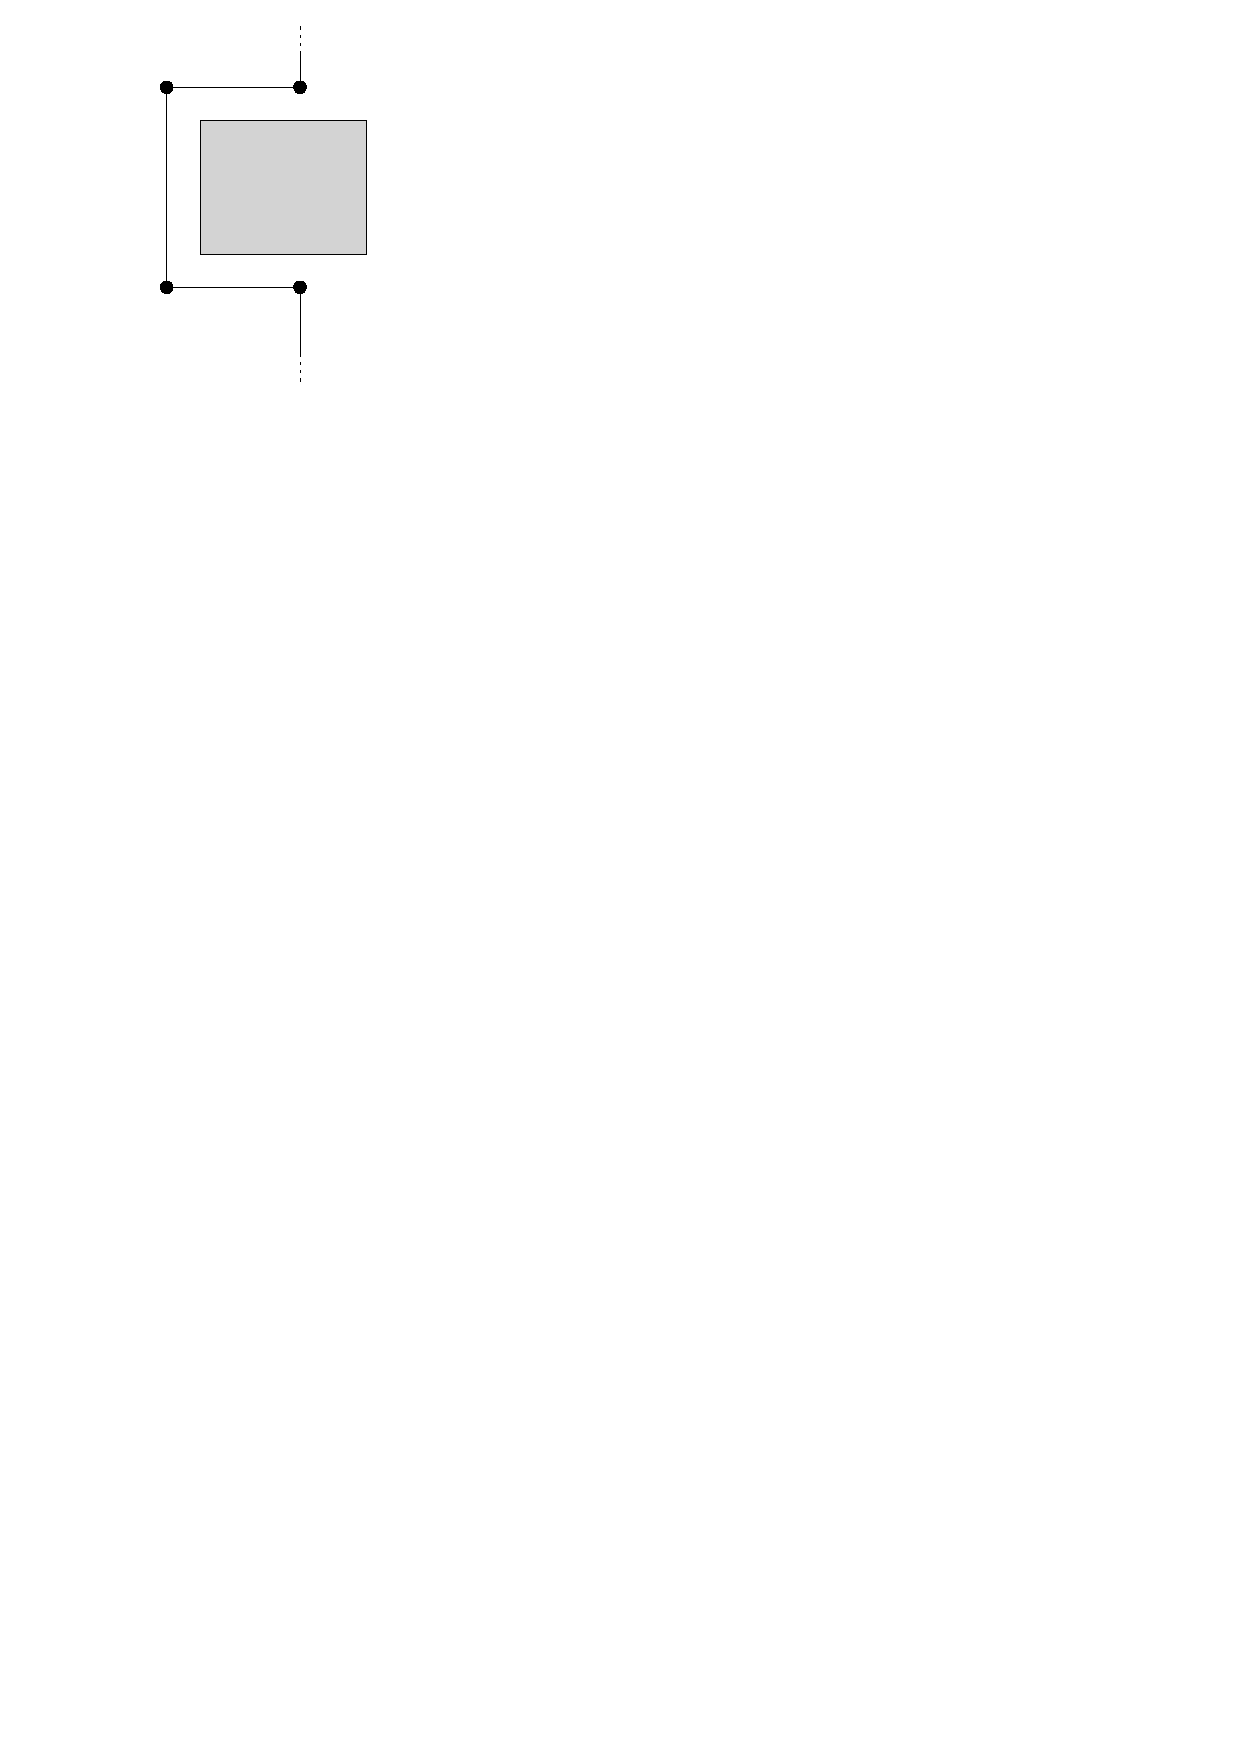
\includegraphics[width=.8\linewidth]{figures/umlauf.pdf}
	\caption{Umlaufung}
	\label{fig:goaround}
\end{minipage}%
\begin{minipage}{.8\textwidth}
  \centering
  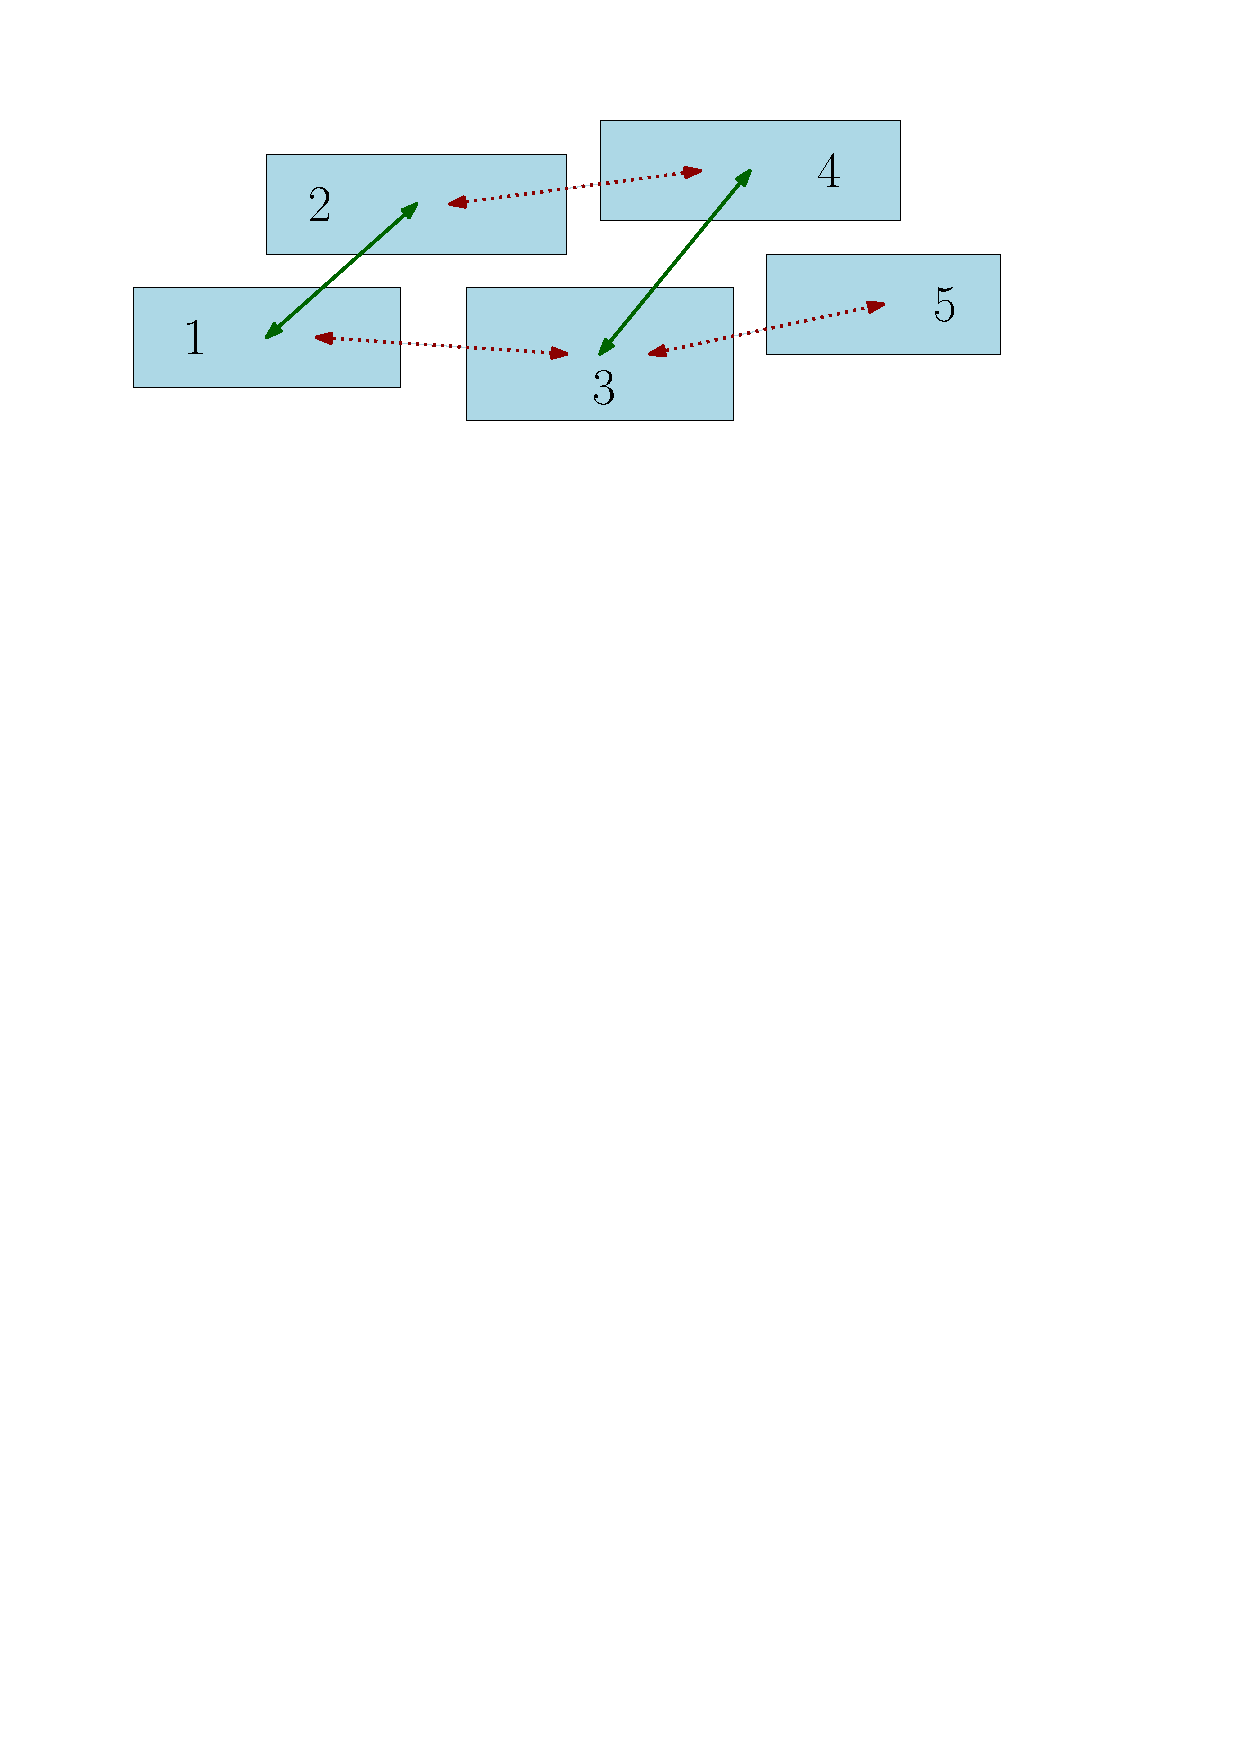
\includegraphics[width=.8\linewidth]{figures/neighbors.pdf}
  \captionof{figure}{Nachbarn}
  \label{fig:neighbors}
\end{minipage}
\end{figure}

Diese Modellierung erlaubt noch keine Knicke zusätzlich zu denen, die schon im Ausgangslayout vorhanden sind. Dies ließe sich umsetzen, indem auf jedem Abschnitt einer Kante zusätzliche Pseudoknicke eingefügt werden, die vom ILP dann genutzt werden können. Zur Knickminimierung ist es hilfreich, die Anzahl der genutzten Pseudoknicke in die Optimierungsfunktion mit aufzunehmen. Es bietet sich an, pro Abschnitt $4$ solcher Pseudoknicke einzufügen, da mit $4$ Knicken in jedem Fall ein Knoten umlaufen werden kann, wie in Abbildung \ref{fig:goaround} zu sehen. Sollten für ein optimales Ergebnis mehr als $4$ zusätzliche Knicke auf einem Kantenabschnitt benötigt werden, so ist eine Lösung ähnlich der in Abschnitt \ref{sub:impl:opt} für die Bedingungen zur Überlappungsfreiheit vorgestellten denkbar: Stellt man nach der Lösung des ILPs fest, dass alle Pseudoknicke auf einem Abschnitt verwendet wurden, so fügt man in die neu entstandenen Abschnitte wiederum je $4$ Pseudoknicke ein und lässt das ILP erneut lösen.

Offensichtlich steigert diese Art Kantenroutings zu betrachten die Komplexität des ILPs noch einmal beträchtlich. Wir haben daher Zweifel daran, dass dies in der Praxis eine nützliche Erweiterung der vorgestellten ILPs ist.
